\chapter{实验与评估}
    \label{sec:experiment}

    本工作的原型系统在三个实际的web API服务上进行了实验, 从四个方面评估了本文提出的场景模型和测试方法: 测试用例多样性, 测试覆盖率, 故障检测能力, 以及测试效率.
    
    \section{实验配置}
        实验选择的第一个被测系统为合作研究组开发的云对象存储服务(OSS)的系统原型(后文简称\textbf{OSS}). 此服务提供了33个web API接口, 并有较完整的使用文档. 测试时, 期望所有的API和功能点都业已实现完成.
        
        最近以来, 云对象存储服务(OSS)已经成为了流行的云存储服务形式. 许多大型云服务提供商均已提供云对象存储服务, 如亚马逊AWS\footnote{https://aws.amazon.com/s3}, IBM云\footnote{ https://console.bluemix.net/catalog/services/cloud-object-storage}和阿里云\footnote{ https://www.alibabacloud.com/product/oss}等. 在云对象存储服务中, 每个账号, 在每个服务器区域, 都可以有许多桶(bucket). 桶(bucket)与文件系统中的文件夹类似, 对象(object)与文件系统中的文件类似. 用户可以上传对象, 删除对象, 重命名对象, 创建符号链接等等. 每个对象都属于一个固定的桶.
        
        对于云对象存储服务, 本工作首先为这33个API编写了OpenAPI格式的API行为描述脚本. 然后, 设计了一些小型场景模型来检验每个API的基本功能. 在此之后, 设计了三个较大型的综合场景模型Scenario A(详见附录图\ref{fig:oss_scenario_A})、Scenario B(详见附录图\ref{fig:oss_scenario_B})、Scenario C(详见附录图\ref{fig:oss_scenario_C})以进行综合测试, 这三个场景均与实际使用场景较相似, 测试用例的生成与执行期望能够模拟实际部署后的高负载环境. 对于每个场景, 运行工具原型随机生成并执行了1,000个测试用例. 所有测试用例及其执行结果都被妥善保存. 后续分析时, 在所有测试用例上进行统计, 而没有进行任何遴选.
        
        第二个被测系统为阿里云的云服务器(ECS)服务(后文简称\textbf{ECS}), 阿里云是世界领先的云计算服务商, 淘宝、12306网站等大型应用均依托阿里云提供计算支持. 
        
        本实验测试阿里云服务为普通用户提供的云计算实例租用服务, 相关接口共有26个, 均为web API, 并配有专业使用文档. 在此服务中, 用户可以租用示例, 退租示例, 获取实例运行状态, 启动示例, 关闭示例, 重启示例等等. 我们选择了其中8个web API, 编写了行为描述脚本, 然后设计了包含所有这8个web API的综合场景模型(详见附录图\ref{fig:ecs_scenario})进行测试. 一共随机生成并执行了100个测试用例, 所有测试用例在进行统计与分析时均纳入考虑.
        
        第三个被测系统是工业界合作团队提供的电子支付服务(后文简称\textbf{E-payment}). 本实验测试它的实时贷记API接口. 此API仅用于系统内部使用, 是微服务之间的通信接口, 因此使用LAN上的定制协议交互. 作为电子支付接口, 此服务拥有很高的可用率与很低的容错率要求. 同时, 它有多达20个参数. 由于模拟环境的缺失, 在本实验中, 暂未进行实际的调用与发送, 而是根据接口描述文档进行测试用例和请求数据的生成, 来验证生成的测试用例可以有效覆盖参数组合, 从而验证其在这类服务的测试上的可用性.
        
        对于E-payment服务, 实验中生成了巨量(超过两百万个)的测试用例, 并计算了这些测试用例对于参数组合的覆盖率. 这种方式不仅仅评估了测试用例的覆盖率, 也检验了工具原型的鲁棒性和性能. 使用的场景主要进行基于数据分区的请求参数生成和参数合成操作, 详见附录图\ref{fig:epayment_scenario}.
        
    
    \section{测试用例多样性}
        富有多样性的测试用例是本文测试方法追求的目标之一. 多样性保证了测试用例集构成的测试套件具有较高的覆盖率和较低的冗余度. 另一方面, 使用被测系统的用户形形色色, 实际的系统负载也十分富有多样性, 因此, 测试用例富有多样性, 在某种程度上也能说明生成它们的测试场景模型可以很好地表达使用场景.
        
        \begin{figure}[!htb]
            \begin{minipage}{0.5\textwidth}
                \centering
                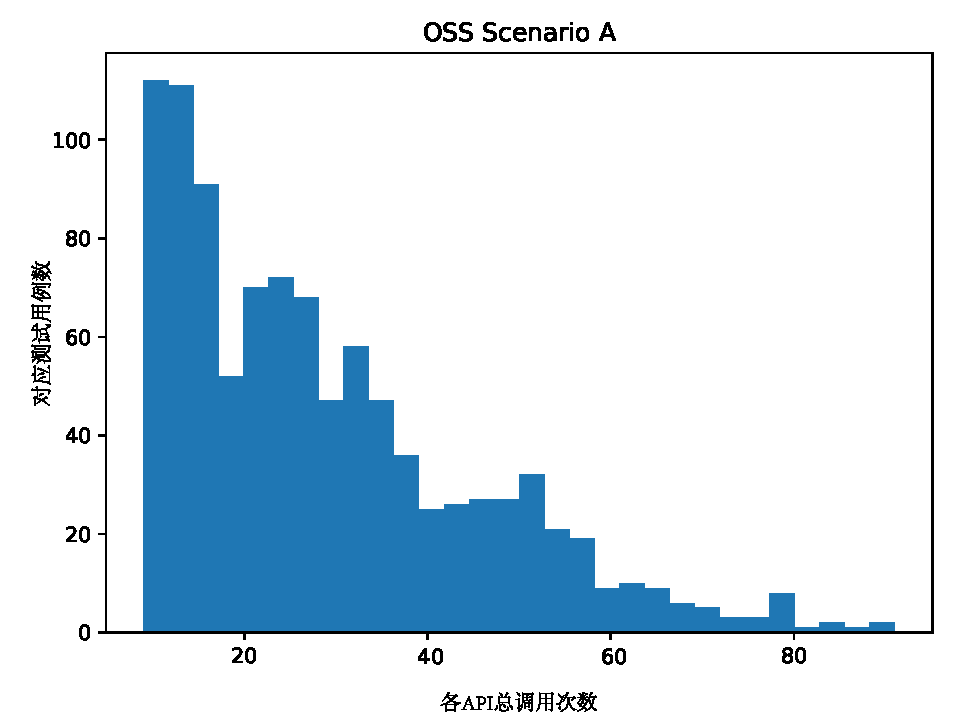
\includegraphics[width=200pt]{OSS_A_APICalls_cn.pdf}
                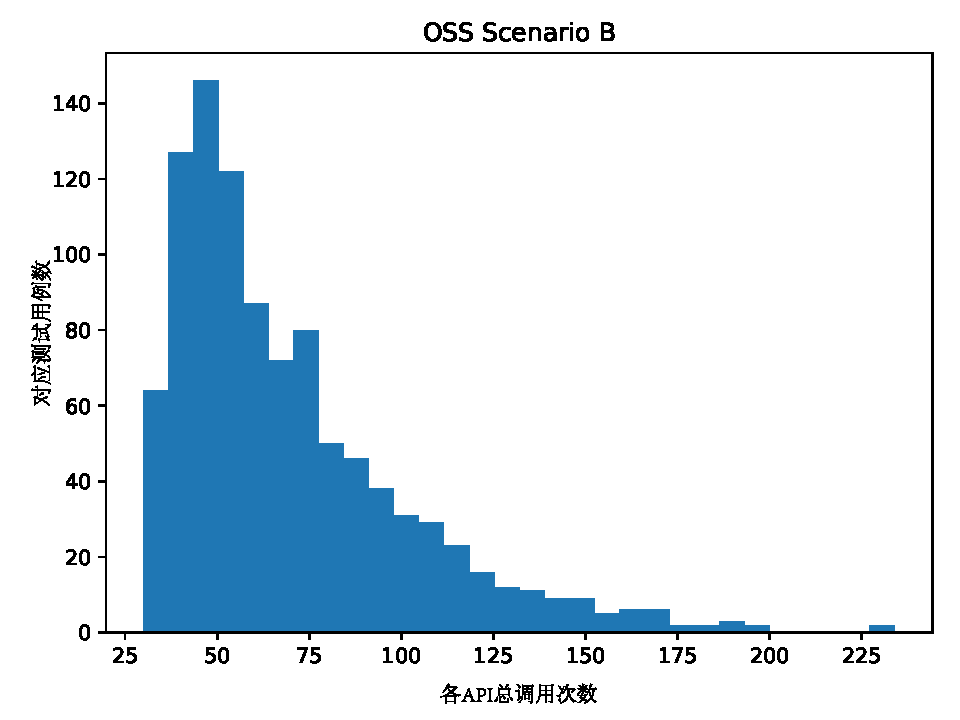
\includegraphics[width=200pt]{OSS_B_APICalls_cn.pdf}
                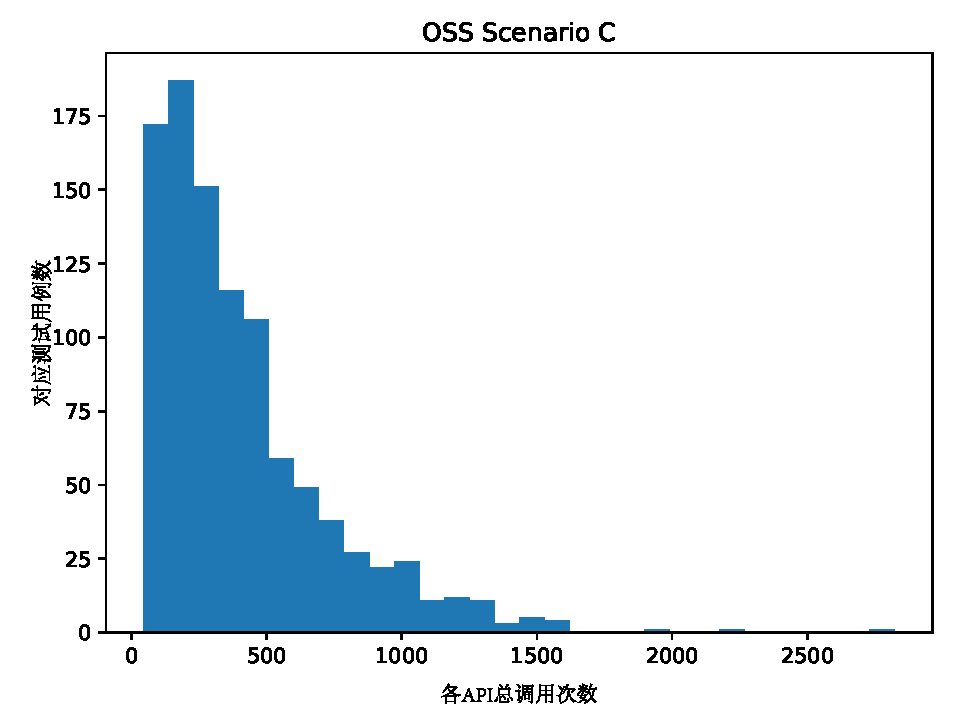
\includegraphics[width=200pt]{OSS_C_APICalls_cn.pdf}
            \end{minipage}
            \begin{minipage}{0.5\textwidth}
                \centering
                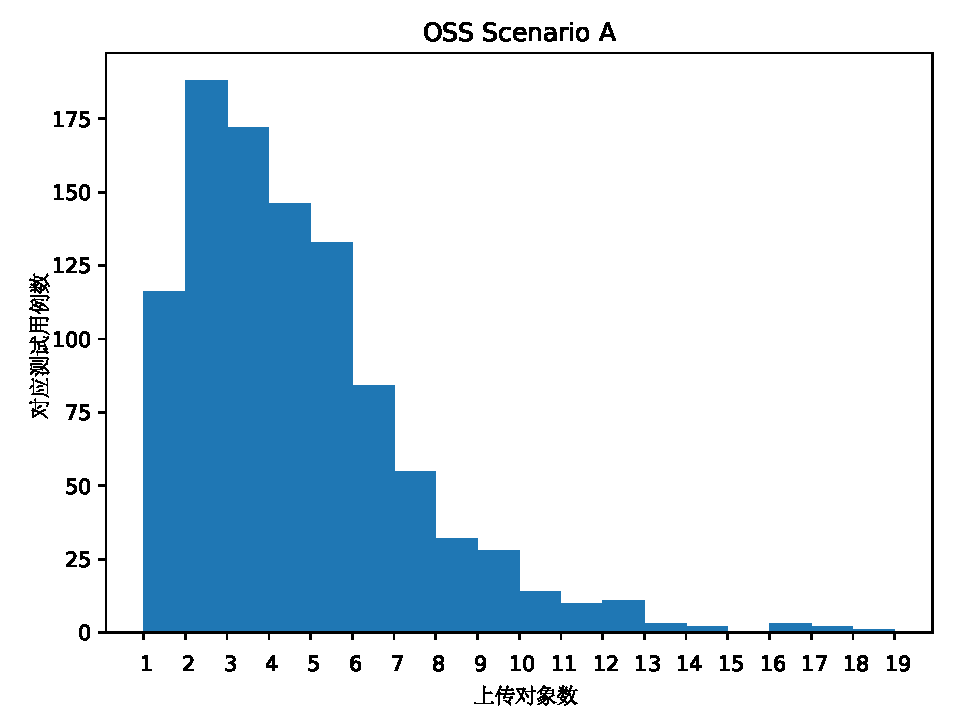
\includegraphics[width=200pt]{OSS_A_UploadedObj_cn.pdf}
                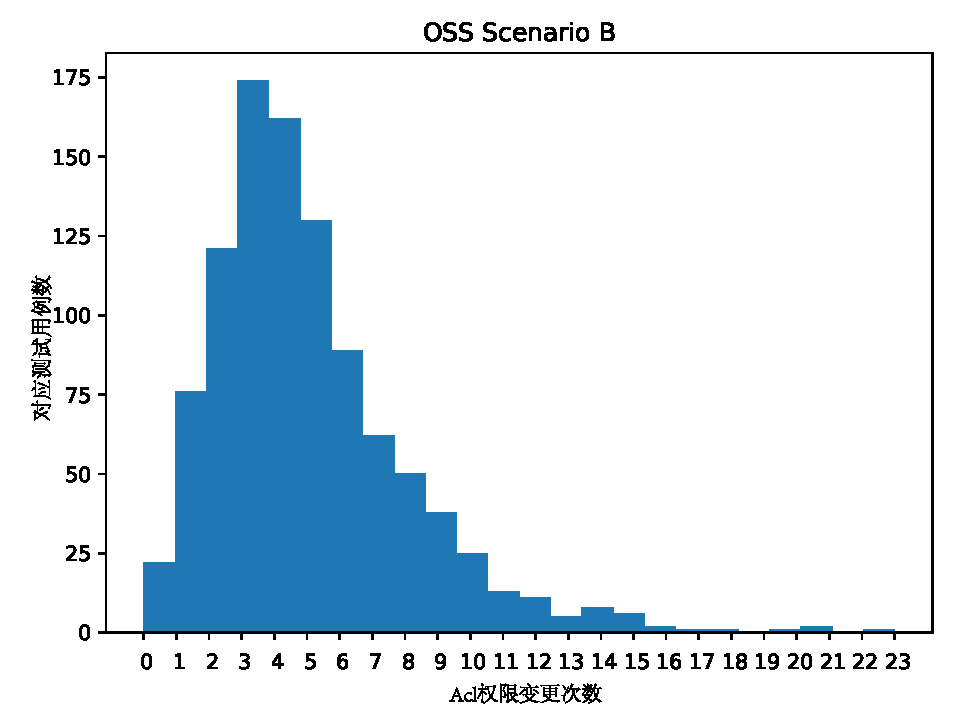
\includegraphics[width=200pt]{OSS_B_AclChange_cn.pdf}
                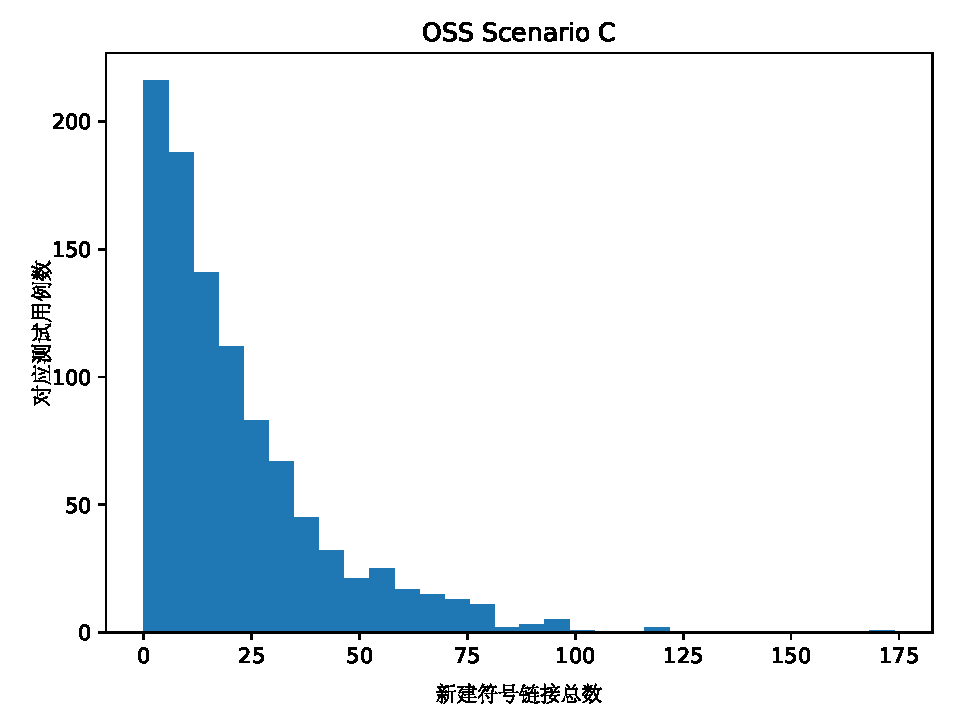
\includegraphics[width=200pt]{OSS_C_Putsymlink_cn.pdf}
            \end{minipage}
            \caption{OSS测试用例操作次数统计直方图. 基于Scenario A, Scenario B, Scenario C三个场景生成的1,000个测试用例. 左侧为每个测试用例调用API的总次数直方图, 右侧对每个场景选取一种典型API, 统计其调用次数直方图.}
            \label{fig:OSS_stat}
        \end{figure}
        
        \begin{figure}[!htb]
            \centering
            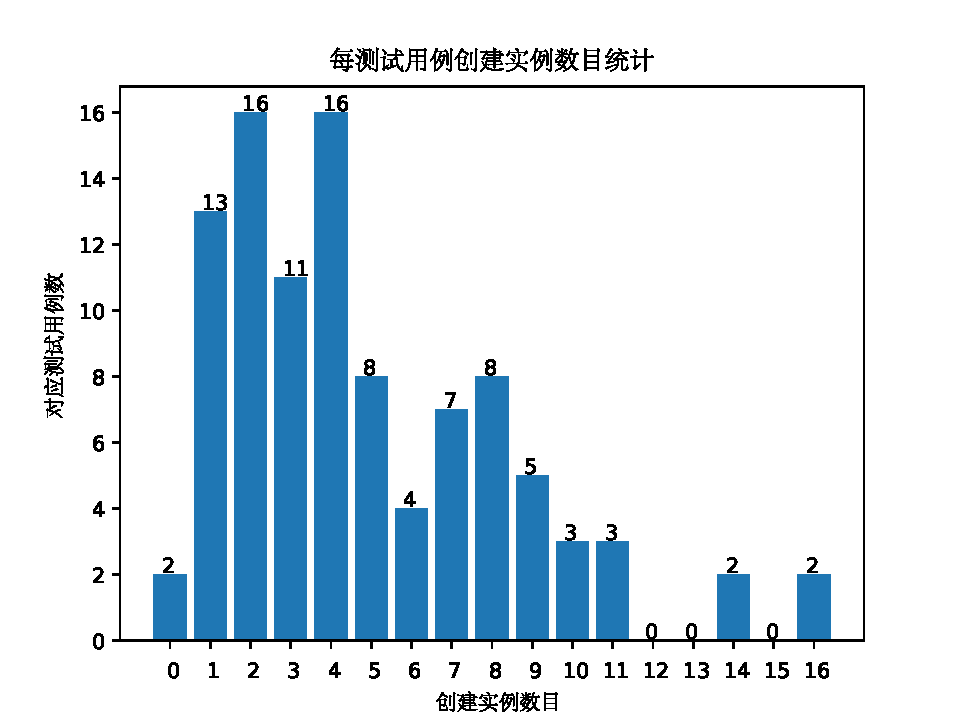
\includegraphics[width=200pt]{EC_instance_distribution_cn.pdf}
            \caption{ECS测试用例实例创建数直方图. 基于ECS测试场景生成的100个测试用例.}
            \label{fig:ECS_stat}
        \end{figure}
        
        在web API测试中, 测试用例的多样性可以通过很多不同的指标反映出来. 图\ref{fig:OSS_stat}反映了对于OSS服务, 生成的测试用例的总API调用次数和典型单API调用次数的统计分布情况. 图\ref{fig:ECS_stat}反映了对于ECS服务, 生成的测试用例创建的实例数的统计分布情况. 虽然由于不同API在场景中所处位置不同的原因, 每副直方图中的分布区间差异较大, 但是整体分布模式是类似的, 即无论是API总调用数目, 单API调用数目, 还是实例创建数目, 分布均较分散. 这反映了生成的测试用例的多样性.
        
        值得注意的是, 虽然这些直方图反映的分布都与指数分布较为接近, 但这只是因为, 在这些场景中大体模式均为一个总状态连接到调用各API的分状态, 并拥有不为零的终止概率, 因此测试用例中各API的调用次数才近似于指数分布. 对于其他场景模式, 其余分布模式当然是完全可能出现的.

    \section{测试覆盖率}
        覆盖率是软件测试中的一项重要指标. 存在许多类型的覆盖率. 在规范导向的黑盒API测试中, 没有办法获取源代码. 因此, 基于源代码的代码覆盖率指标和分支覆盖率指标无法使用. 此处使用的覆盖率指标主要为API覆盖率和数据分区组合的覆盖率.
        
        
    
    \section{故障检测能力}
    
    \section{测试效率}

